\documentclass[a4paper,
    11pt,
    headings=small,
    ngerman,
    listof=totoc,
    numbers=noenddot]{scrreprt}[2021/11/13]
\usepackage{ifxetex,ifluatex}
\ifcase \ifxetex 1\else\ifluatex 1\else 0\fi\fi\usepackage[utf8]{inputenc}\fi
\usepackage[T1]{fontenc}
\usepackage[ngerman]{babel}
\usepackage[utf8]{inputenc}
\usepackage{setspace}
\onehalfspacing
\usepackage{lmodern}
\usepackage{csquotes}

\usepackage[automark,headsepline=.4pt]{scrlayer-scrpage}
\clearmainofpairofpagestyles
\pagestyle{scrheadings}
\renewcommand*{\chaptermarkformat}{%
	\chaptername~\thechapter\autodot\enskip}
\ihead{\headmark}
\setkomafont{pageheadfoot}{}
\renewcommand*{\sectionmarkformat}{}
\cfoot{\pagemark}
\footskip1cm

\usepackage[left=2.5cm,right=2.5cm,top=3cm,bottom=2.5cm]{geometry}

\usepackage{xcolor, soul}
\definecolor{codebackground}{rgb}{0.95, 0.95, 0.92}
\definecolor{Black}{rgb}{0, 0, 0}

%%% Für Abkürzungen und Abkürzungsverzeichnis %%%
\usepackage[printonlyused,withpage]{acronym}

%%% Für Mathe %%%
\usepackage[fleqn]{amsmath}
\usepackage{commath}
\usepackage{amstext}
\allowdisplaybreaks
%%% Für schräge Bruchstriche %%%
\usepackage{nicefrac}

%%% Für Quotes %%%
\usepackage{url}
\usepackage[ngerman]{varioref}
\usepackage{mwe}
\usepackage{hyperref}% Weil es so in der Frage enthalten war.
 \hypersetup{%draft, 								% no hyperlinking at all (useful in b/w printouts)
    colorlinks=true, breaklinks=true,
    urlcolor=Black, linkcolor=Black, citecolor=Black,
    linktoc=page, %
    bookmarksnumbered, bookmarksopenlevel=1, bookmarksdepth = section,%
    pdfstartview=FitV,
    }
\setlength{\parindent}{0em}
\usepackage{bookmark}% Weil das hyperref deutlich verbesser.
\usepackage{cleveref}
\crefname{paragraph}{Abschnitt}{Abschnitt}
\crefname{lstlisting}{Listing}{Listings}

%%% Für Textübergreifende Numerierung %%%
\usepackage{enumitem}
\renewcommand{\labelenumi}{\alph{enumi})}

%%% Um PDFs einzubinden %%%
\usepackage{pdfpages}

%%% Um Zahlen mit Einheiten korrekt darstellen %%%
\usepackage{siunitx}
\sisetup{
  locale = DE ,
  detect-all,
  binary-units = true
}

%%% Code schoen darstellen %%%
\usepackage{listings}
\lstdefinestyle{MyPythonStyle}{
  frame=tb, % hrule above and below
  keepspaces=true,
  breaklines=true,
  columns=flexible,
  basicstyle=\texttt\scriptsize,
  escapeinside={(*@}{@*)}, % for escaping
  backgroundcolor=\color{codebackground},
  showstringspaces=false,
  language=Python,
  keywordstyle=\color{blue},
  stringstyle=\color{red},
  commentstyle=\color{teal},
  numbers=left, % {none, left, right}
  firstnumber=1,
  numberstyle=\scriptsize\color{black},
  numbersep=5pt,
  xleftmargin=5.0ex,
  gobble=-4
}

%%% Korrekte darstellung fuer Sonderzeichen im Code
\lstset{literate=%
    {Ö}{{\"O}}1
    {Ä}{{\"A}}1
    {Ü}{{\"U}}1
    {ß}{{\ss}}1
    {ü}{{\"u}}1
    {ä}{{\"a}}1
    {ö}{{\"o}}1
    {~}{{\textasciitilde}}1
}


%%% Verzeichnisse im Anhang %%%
\DeclareNewTOC[%
  owner=\jobname,
  listname={Inhalt des Anhangs},% Titel des Verzeichnisses
]{atoc}% Dateierweiterung (a=appendix, toc=table of contents)
\DeclareNewTOC[%
  listname={Abbildungen im Anhang},% Titel des Verzeichnisses
]{alof}% Dateierweiterung (a=appendix, lof=list of figures)
\DeclareNewTOC[%
  listname={Tabellen im Anhang},% Titel des Verzeichnisses
]{alot}% Dateierweiterung (a=appendix, lot=list of tables)
 
\makeatletter
\newcommand*{\useappendixtocs}{%
  \renewcommand*{\ext@toc}{atoc}%
  \scr@ifundefinedorrelax{hypersetup}{}{% damit es auch ohne hyperref funktioniert
    \hypersetup{bookmarkstype=atoc}%
  }%
  \renewcommand*{\ext@figure}{alof}%
  \renewcommand*{\ext@table}{alot}%
}
\newcommand*{\usestandardtocs}{%
  \renewcommand*{\ext@toc}{toc}%
  \scr@ifundefinedorrelax{hypersetup}{}{% damit es auch ohne hyperref funktioniert
    \hypersetup{bookmarkstype=toc}%
  }%
  \renewcommand*{\ext@figure}{lof}%
  \renewcommand*{\ext@table}{lot}%
}
\scr@ifundefinedorrelax{ext@toc}{%
  \newcommand*{\ext@toc}{toc}
  \renewcommand{\addtocentrydefault}[3]{%
    \expandafter\tocbasic@addxcontentsline\expandafter{\ext@toc}{#1}{#2}{#3}%
  }
}{}
\makeatother
 
\usepackage{xpatch}
\xapptocmd\appendix{%
  \addpart{\appendixname}
  \useappendixtocs
}{}{}

%%% Alles bzgl. des Literaturverzeichnisses
\usepackage[bibencoding=utf8,
			sortlocale=de,
			style=numeric,
			pagetracker=true,
			autocite=inline,
			backrefstyle=three+,
			date=short,
			sorting=nty,
			backend=biber]{biblatex}
\bibliography{Literaturverzeichnis}

%%% urldate in eckigen Klammern %%%
\DeclareFieldFormat{urldate}{\mkbibbrackets{#1}}
%%% URL: = Verfügbar unter: %%%
\DeclareFieldFormat{url}{{Verfügbar unter:}\space\url{#1}}
%%% Abstand zwischen den Literaturangaben %%%
\setlength{\bibitemsep}{1.3em}
%%% statt und ein & %%%
\renewcommand*{\finalnamedelim}{\space\&\space}
%%% Nachname, Vorname, immer %%%
\DeclareNameAlias{sortname}{last-first}

\begin{document}
\pagenumbering{gobble}
\pagestyle{empty}


\begin{center}
  \Large{Berufliches Schulzentrum für Elektrotechnik Dresden}\\
\end{center}

\begin{center}
  \Large{Fachbereich Informationstechnik}
\end{center}
\begin{verbatim}

\end{verbatim}
\begin{center}
  \textbf{\LARGE{Projektdokumentation}}
\end{center}

\begin{center}
  \Large{Lernfeld 9 - Projekt 3}
\end{center}

\vspace{\fill}

\begin{flushleft}
  \begin{tabular}{lll}
                            &                                                & \\
                            &                                                & \\
                            &                                                & \\
                            &                                                & \\
                            &                                                & \\
                            &                                                & \\
    \textbf{Auftraggeber:}  & Doubtful-Joy SE                                & \\
    \textbf{Auftragnehmer:} & High-Secure GmbH - Projektteam IT20/2 Gruppe 7 & \\
    \textbf{Auftragsdatum:} & 2021.11.15                                     & \\
                            &                                                & \\
    \textbf{Historie:}
                            &                                                  \\
                            &                                                & \\
  \end{tabular}
\end{flushleft}

%%% Inhaltsverzeichnis
\tableofcontents

\newpage

%%% Abkürzungsverzeichnis %%%
\chapter*{Abkürzungsverzeichnis}
\addcontentsline{toc}{chapter}{Abkürzungsverzeichnis}

\begin{acronym}[DHCP]
  \acro{API}{Application Programming Interface}
  \acro{CRUD}{create, read, update und delete}
  \acro{DB}{Datenbank}
  \acro{DHCP}{Dynamic Host Configuration Protocol}
  \acro{DNS}{Domain Name System}
  \acro{DMZ}{Demilitarisierte Zone}
  \acro{SSH}{Secure Shell}
  \acro{VM}{virtuelle Machine}
  \acrodefplural{VM}{virtuelle Machinen}
\end{acronym}

\newpage
\pagestyle{scrheadings}
\pagenumbering{arabic}
\ohead{Projekt 3, Lehrjahr 21/22}
\ihead{\rightmark}


\chapter{Pflichtenheft}



\section{Auftraggeber und Auftragnehmer }

Beim Auftraggeber handelt es sich um die Gaming-Plattform \textbf{Doubtful-Joy SE}. Ansprechpartner sind

\begin{table}[htbp]
  \centering
  \renewcommand{\arraystretch}{1.25}
  \caption{Ansprechpartner Auftraggeber}
  \begin{tabular}{lllll}
    Funktion     & Name   & Vorname & Email                                 \\
    \hline
    Auftraggeber & Hempel & Steffen & \flq{}hempel@bszetdd.lernsax.de\frq{} \\
  \end{tabular}
  \label{tab:Auftraggeber}
\end{table}

Beim Auftragnehmer handelt es sich um das \textbf{High-Secure GmbH - Projektteam IT20/2 Gruppe 7}. Ansprechpartner sind

\begin{table}[htbp]
  \centering
  \renewcommand{\arraystretch}{1.25}
  \caption{Ansprechpartner Auftragnehmer}
  \begin{tabular}{lllll}
    Funktion          & Name      & Vorname  & Email                                         \\ \hline
    Projektmanager    & Egermann  & Péter    & \flq{}i20egermannpe@bszetdd.lernsax.de\frq{}  \\
    Teamleiter        & Leyrer    & Johannes & \flq{}i20leyrerjo@bszetdd.lernsax.de\frq{}    \\
    Netzwerkingenieur & Brethfeld & Vinzenz  & \flq{}i20brethfeldvi@bszetdd.lernsax.de\frq{} \\
  \end{tabular}
  \label{tab:Auftragnehmer}
\end{table}



\section{Ausgangslage}

Die existierende Support-Infrastruktur der Gaming-Plattform Doubtful-Joy SE lässt sich über Mail und Telefon kontaktieren. Dabei wird jeder Anruf und jede Mail individuell von einem Mitarbeiter als Ticket gespeichert und in einem zentralen Laufwerk abgelegt. Effizienz, Ordnung und Übersichtlichkeit sind nicht ausreichend vorhanden.



\section{Projektziel}

Die Gaming-Plattform Doubtful-Joy SE möchte ihre existierende Support-Infrastruktur durch ein Ticketsystem ersetzen. Dieses soll für Kunden und Mitarbeiter über ein Web-Interface erreichbar sein. Tickets sollen über dieses direkt erstellt und mit beliebig vielen Attachments versehen werden können.

Außerdem soll eine Segmentierung der Netzinfrastruktur mit einer sichereren Trennung von öffentlich erreichbaren Diensten und dem Intranet eingerichtet werden. Ebenso sollen die internen Dienste \ac{DNS} und \ac{DHCP} auf einem separatem System bereitgestellt werden, um eine Abhängigkeit von der Firewall auszuschließen.

Doubtful-Joy SE setzt auf RedHat und binärkompatible Systeme, weshalb diese System-Strategie weiterhin umgesetzt werden soll.



\section{Funktionsspezifikation}

Von der Realisierung sind betroffen:

\begin{description}
  \item[Manware] \
    \begin{itemize}
      \item Projektteam IT20/2 Gruppe 7
      \item Support-Mitarbeiter des Auftraggeber
      \item IT-Mitarbeiter des Autraggebers
    \end{itemize}
  \item[Orgware] \
    \begin{itemize}
      \item Sicherheitsanforderungen
      \item Benutzerhandbuch
      \item Benutzerschulung
    \end{itemize}
  \item[Hardware] \
    \begin{itemize}
      \item Server
      \item Mitarbeiter-PCs
    \end{itemize}
  \item[Software] \
    \begin{itemize}
      \item VM-Ware
      \item Datenbank-Server
      \item Web-Server
      \item Firewall-System
      \item \ac{DNS}
      \item \ac{DHCP}
    \end{itemize}
\end{description}



\section{Datenspezifikation}

Da von etwa 1000 Telefonanrufen  und Emails pro Tag ausgegangen wird, kann dies etwa 1:1 in 1000 Tickets übertragen werden. Der Speicherbedarf pro Ticket wird hier im Schnitt auf etwa \SI{5}{\mega\byte} geschätzt, da wahrscheinlich häufiger Anhänge in Bildform zur besseren Problembeschreibung genutzt werden. Zusätzlich wird davon ausgegangen, dass die Daten zur Sicherheit und Nachvollziehbarkeit für ein Jahr gespeichert werden, wodurch die Datenbank \SI{1830}{\giga\byte} Speicher in einem Jahr benötigt.

\begin{align*}
  \frac{\SI{5}{\mega\byte}}{\text{Ticket}} \cdot \frac{1000\text{ Ticket}}{\text{Tag}} & = \frac{\SI{5000}{\mega\byte}}{\text{Tag}}                                                                  \\
  \frac{\SI{5000}{\mega\byte}}{\text{Tag}} \cdot 365 \text{Tage}                       & = \frac{\SI{1825000}{\mega\byte}}{\text{Jahr}} \stackrel{\wedge}= \frac{\SI{1830}{\giga\byte}}{\text{Jahr}}
\end{align*}


Da es keine Good-Practice ist, die Bilder in der Datenbank zu speichern, wird nur der Dateipfad zu den Bildern in der Datenbank hinterlegt, die Bilder selbst liegen auf der Festplatte des Webservers. Damit verringert sich der geschätzte Speicherbedarf der Datenbank auf etwa \SI{183}{\giga\byte} pro Jahr.

\begin{align*}
  \frac{\SI{0.5}{\mega\byte}}{\text{Ticket}} \cdot \frac{\text{Ticket}}{\text{Tag}} = \frac{\SI{500}{\mega\byte}}{\text{Tag}} \stackrel{\wedge}= \frac{\SI{183}{\giga\byte}}{\text{Jahr}}
\end{align*}

Die Bilder selbst benötigen zum aktuellen Stand auf der Festplatte \SI{1643}{\giga\byte} Speicher pro Jahr.

\begin{align*}
  \frac{\SI{4.5}{\mega\byte}}{\text{Bild}} \cdot 1000 \frac{\text{Bild}}{\text{Tag}} = \frac{\SI{4500}{\mega\byte}}{\text{Tag}} \stackrel{\wedge}= \frac{\SI{1643}{\giga\byte}}{\text{Jahr}}
\end{align*}

Die Art von Daten sind personenbezogene Daten in Text- und Bildform.

Der Datenfluss geht vom Clienten zur \ac{DMZ} und zur Bearbeitung dann zum PC des Support-Mitarbeiters, grafisch dargestellt in \vref{fig:Schnittstellenspezifikation}.



\newpage
\section{Schnittstellenspezifikation}

\begin{figure}[htbp]
  \centering
  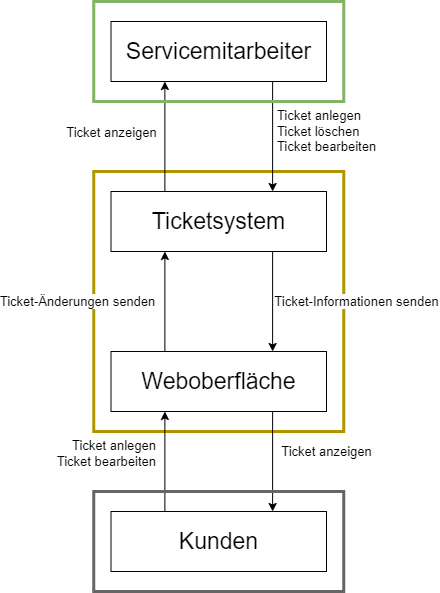
\includegraphics[width=0.75\textwidth]{data/Schnittstellendiagramm.png}
  \caption{Schnittstellenspezifikation}
  \label{fig:Schnittstellenspezifikation}
\end{figure}



\section{Rahmenbedigungen}

Der Auftraggeber hat folgende Ressourcen bereitzustellen und Mitwirklungspflichten:

\begin{itemize}
  \item Server
  \item Mitarbeiter-PCs
  \item Zugriff auf alle zu bearbeitenden Systeme und Zutritt zu den notwendigen Räumlichkeiten
  \item Kooperation und eventuell notwendigen lokalen Support
\end{itemize}



\section{Qualitätsbetrachtung}

Die Arbeitspakete werden stets während der Bearbeitung sowie nach der Fertigstellung auf Funktion und Qualität überprüft.

Wöchentlich werden Meetings abgehalten um den Stand des Projekts zu erörtern und auf eventuell auftretende Probleme zeitnah reagieren zu können.

Die Zeitplanung und damit der Aufwand ist in \vref{fig:GanttKlein} in kleinem Format und groß in \vref{fig:Gantt} zu sehen.  Für einen langfristigen Support für nach der der Fertigstellung wird ein zusätzliches Angebot vorgelegt.



\section{Projektplanung}

Die Projektplanung ist im Projektstrukturplan, zu sehen in \vref{fig:Projektstrukturplan}, und im Gantt-Diagramm, zu sehen in \vref{fig:GanttKlein}, bzw. \vref{fig:Gantt}, abgebildet.
Ebenso wird der im Anhang \cpageref{fig:Netzwerkplan} zu betrachtende Netzwerkplan \vref{fig:Netzwerkplan} umgesetzt.

\begin{figure}[htbp]
  \centering
  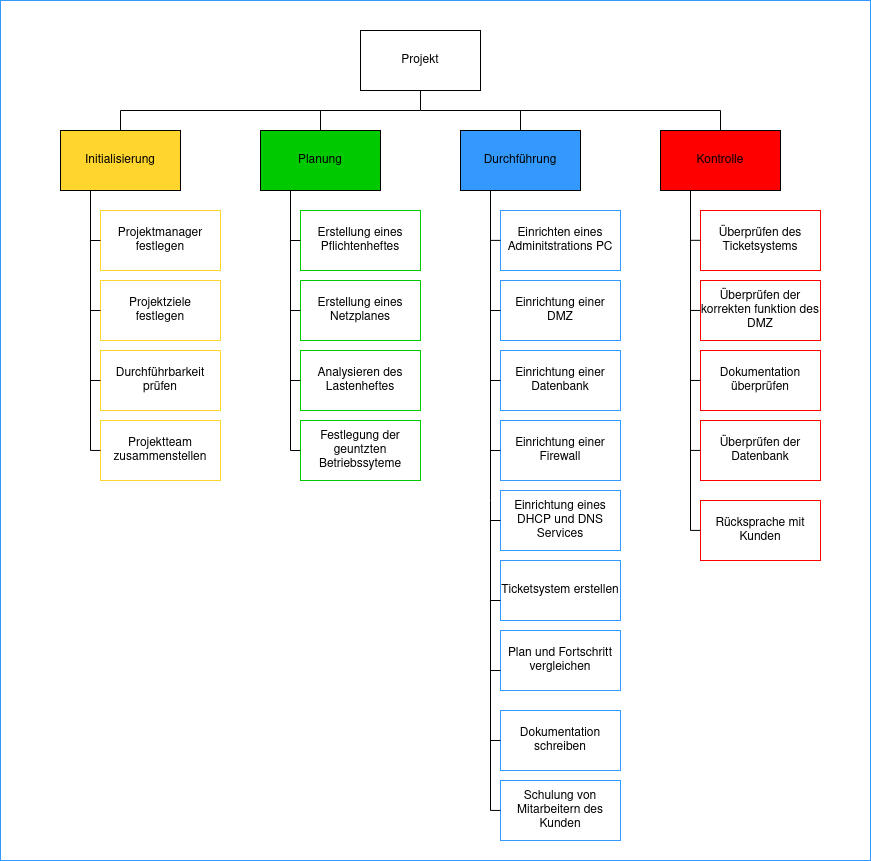
\includegraphics[width=0.75\textwidth]{data/Projektstrukturplan.png}
  \caption{Projektstrukturplan}
  \label{fig:Projektstrukturplan}
\end{figure}

\begin{figure}[htbp]"-
  \centering
  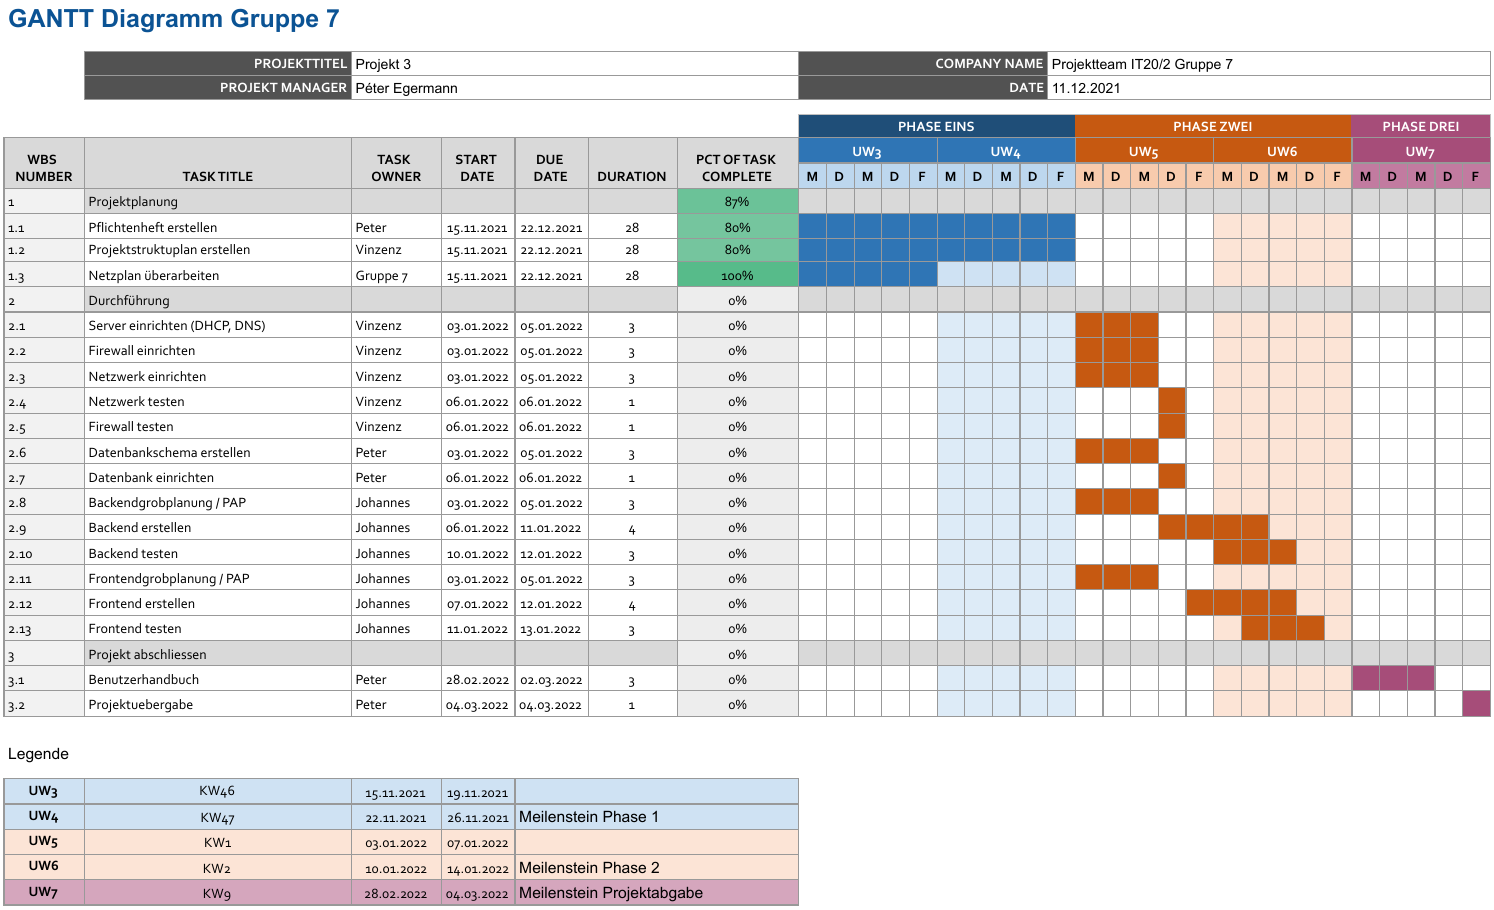
\includegraphics[width=0.95\textwidth]{data/Gantt.png}
  \caption{Gantt-Diagramm}
  \label{fig:GanttKlein}
\end{figure}



\section{Kosten-Nutzen-Analyse}

Eine Kosten-Nutzen-Analyse ist zum jetzigen Zeitpunkt nicht notwendig, da der Support erst mal entlastet werden muss. Dies ist durch das neue System auf jeden Fall der Fall, da quasi der Kunde das Ticket erstellt und nicht der Support-Mitarbeiter. Somit kann sich voll auf das Beheben des Problems konzentriert werden.




\chapter{Auswertung und Reflexion}



\section{Ablaufdokumentation}

In diesem Projekt werden drei virtuelle Netze eingerichtet, um den Aufbau eines echten Netzwerks zu simulieren. Dabei handelt es sich um das rote Netz, das das Internet wiedergeben soll, das orange Netz, was eine sogenannte \ac{DMZ} darstellt und das grüne Netz, welches das interne Netz darstellt.

Um die Kommunikation und den Zugriff zwischen den Netzen zu regeln wird in diesem Projekt die Firewall verwendet. Somit kann aus dem roten Netz nur mit dem orangen Netz kommuniziert werden, aus dem grünen Netz ist kein Zugriff auf das Internet möglich und zwischen dem orangen und grünen Netz sind nur bestimmte Ports zur Kommunikation und Datenübertragung zugelassen.

Um Maschinen in den verschiedenen Netzen darzustellen wurden vier verschiedene \acp{VM} aufgesetzt, die bis auf die IPFire auf CentOS 8 Stream basieren:

\begin{itemize}
  \item IPFire (als Knotenpunkt für alle drei Netze)
  \item Admin-PC (grünes Netz)
  \item \acs{DHCP}-\acs{DNS}-\acs{DB}-Server (grünes Netz)
  \item Webserver (\ac{DMZ}, oranges Netz)
\end{itemize}



\section{Einrichtung IPFire}

Vor dem Einrichten der IPFire müssen noch zwei Netzwerke zu dem durch VMWare standardmäßig schon bestehenden Netzwerk hinzugefügt werden, da die Firewall mit drei verschiedenen Netzen interagieren soll. Dazu werden den einzelnen Netzen verschiedene MAC-Adressen zugeteilt, damit sie in der späteren Nutzung zuordenbar sind.

Die Netzwerke werden wie in \vref{tab:Netzwerk} zu sehen verteilt.

\begin{table}[htbp]
  \centering
  \renewcommand{\arraystretch}{1.25}
  \caption{Netzwerkauslegung}
  \begin{tabular}{lll}
    Netzwerk-Farbe & MAC-Adresse       & Netzwerk \\
    \hline
    Rot            & 00:50:56:32:BA:0F & NAT      \\
    Grün           & 00:50:56:3D:EC:D6 & VMnet1   \\
    Orange         & 00:50:56:3E:56:B7 & VMnet2   \\
  \end{tabular}
  \label{tab:Netzwerk}
\end{table}

Als Hostname der Firewall wird \glqq{}ipfire\grqq{} und als Domaine \glqq{}doubtful-joy07.com\grqq{} festgelegt.
Nach dem Auswählen der Sprache wird aufgrund der Kundenspezifikation das Filesystem \glqq{}ext4 Filesystem\grqq{} ausgewählt. Nach dem Zuweisen der einzelnen Netze mit den IP- und MAC-Adressen wird der \ac{DHCP} deaktiviert, damit es später mit dem \ac{DHCP}-Server im grünen Netz nicht zu Komplikationen führt.

Nach dem Einrichten der Firewall werden aus dem grünen Netz mittels des IPFire-Web"-interfaces verschiedene Einstellungen der Firewall bearbeitet. Für die Verbindungen zwischen Admin-PC, \ac{DHCP}-\ac{DNS}-\ac{DB}-Server und Webserver sowie für die Erreichbarkeit des Webservers aus dem roten Netz werden vier verschiedene Regeln erstellt, die in \vref{fig:FirewallConfig} zu sehen sind.

\begin{figure}[htbp]
  \centering
  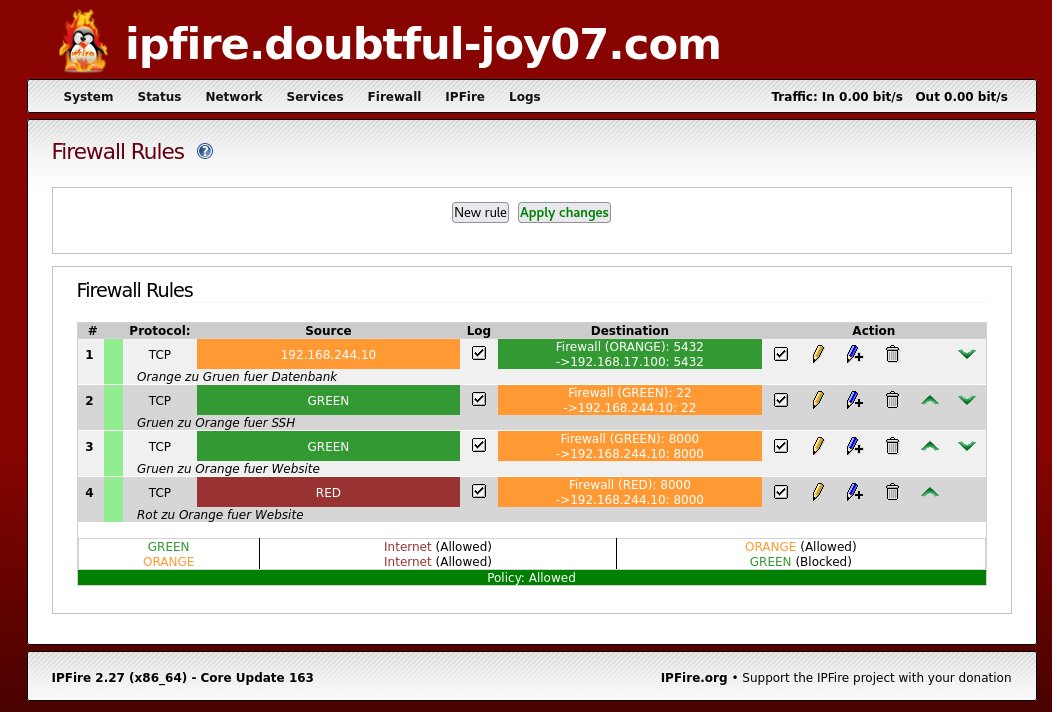
\includegraphics[width=0.95\textwidth]{data/ipfire-config.png}
  \caption{Firewall-Regeln}
  \label{fig:FirewallConfig}
\end{figure}

Die erste Regel dient der Kommunikation zwischen Webserver (\ac{DMZ}) und Datenbank (grünes Netz), sodass Tickets abgerufen und gespeichert werden können. Damit aus dem grünen Netz der Webserver gestartet und gestoppt werden kann, wird Regel 2 implementiert, welche einen \ac{SSH}-Zugang aus dem grünen Netz erlaubt. Die Erreichbarkeit des Webinterface der Ticket-Seite durch die Mitarbeiter aus dem grünen Netz wird mit Regel 3 erreicht. Die letzte Regel erlaubt den Zugriff aus dem Internet auf die Ticket-Website.



\section{Einrichtung Admin-PC}

Nach der Standard-Installation von CentOS 8 Stream wird das Netzwerk der \ac{VM} angepasst. Hier wird der \ac{DNS} auf die IP-Adresse des \ac{DHCP}-\ac{DNS}-\ac{DB}-Servers gesetzt.

Da in CentOS 8 Stream \ac{SSH}-Client und -Server bereits installiert und aktiviert sind, kann der Webserver direkt angesprochen werden. Dies erfolgt über das Gateway des grünen Netzes, wie in \vref{fig:PythonScriptRunning} zu sehen. Um zu sehen, ob der Webserver aktiv ist, können mittels \texttt{ps -ef | grep python} alle laufenden Python-Anwendungen aufgelistet werden, was ebenfalls in \vref{fig:PythonScriptRunning} zu sehen ist.

\begin{figure}[htbp]
  \centering
  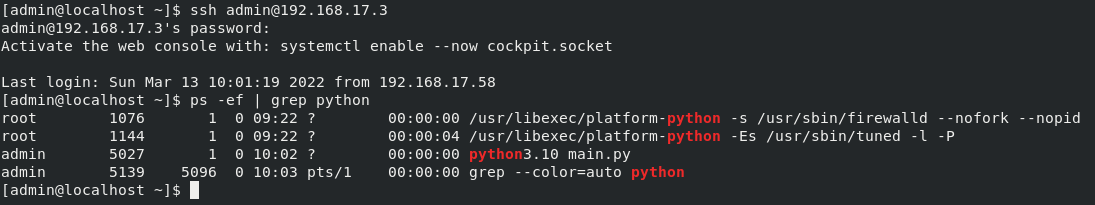
\includegraphics[width=0.95\textwidth]{data/py-script-running.png}
  \caption{\ac{SSH}-Login sowie Auflisten aller laufenden Python-Anwendungen}
  \label{fig:PythonScriptRunning}
\end{figure}

Ist der Webserver aktiv und soll gestoppt werden, kann mittels \texttt{ps -ef | grep python} die ID des Scripts ermittelt und mittels \texttt{kill -9 ID} gestoppt werden. Dies ist in \vref{fig:PythonScriptStop} zu sehen.

\begin{figure}[htbp]
  \centering
  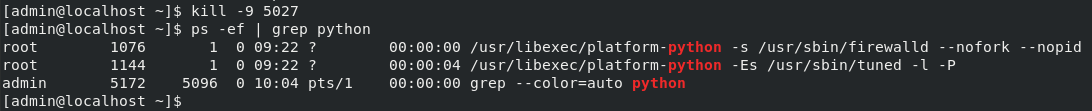
\includegraphics[width=0.95\textwidth]{data/py-script-admin-stop.png}
  \caption{Stoppen einer bestimmten Python-Anwendungen}
  \label{fig:PythonScriptStop}
\end{figure}

Soll der Webserver gestartet werden, kann dies mittels Navigation in den Ordner, in dem die auszuführende Datei liegt und \texttt{python3.10 name-der-datei \&} gestartet werden, zu sehen in der \vref{fig:PythonScriptStart}. Das \& erlaubt das Laufen der Anwendung im Hintergrund und wird so nicht gestoppt, wenn die \ac{SSH}-Verbindung geschlossen wird.

\begin{figure}[htbp]
  \centering
  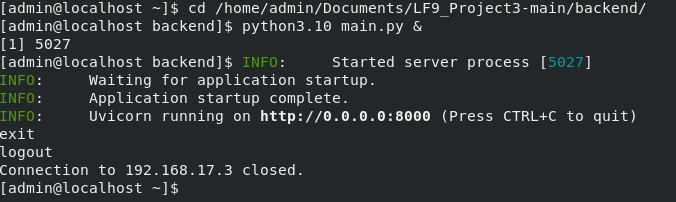
\includegraphics[width=0.95\textwidth]{data/py-script-admin-start.png}
  \caption{Starten einer bestimmten Python-Anwendungen}
  \label{fig:PythonScriptStart}
\end{figure}



\section{Einrichtung DHCP-DNS-DB-Server}


\subsection{Einrichtung der CentOS-Installation}

Wie auch der Admin-PC wird der \ac{DHCP}-\ac{DNS}-\ac{DB}-Server mit CentOS 8 Stream eingerichtet. In den Netzwerkeinstellungen wird die IP-Adresse fest auf \texttt{192.168.17.100}, die Netzwerkmaske auf \texttt{255.255.255.0} und das Gateway auf \texttt{192.169.17.3} gesetzt. Außerdem werden die Dienste \ac{DNS} und \ac{DHCP} in der Firewall freigegeben, zu sehen in \vref{lst:DienstFreigabe}.

\begin{lstlisting}[language=bash,caption={Dienste-Freigabe einer CentOS-Firewall},label={lst:DienstFreigabe}]
  # firewall-cmd --add-service=dns --permanent
  # firewall-cmd --add-service=dhcp --permanent
  # firewall-cmd --reload
\end{lstlisting}


\subsection{Einrichtung des DHCP und DNS}

Die Installation und Einrichtung des \ac{DHCP}s und \ac{DNS} erfolgt mittels der Anleitung für dnsmasq von Michelle Ferron. \autocite{zextras:DHCPDNS}

Die Einstellungen des \ac{DHCP} wird mittels der in \vref{lst:DHCPSettings} zu sehenden Befehle und Einstellungen angepasst.

\begin{lstlisting}[language=bash,caption={DHCP-Einstellungen},label={lst:DHCPSettings}]
  # nano /etc/dnsmasq.conf
  listen-address=::1,127.0.0.1,192.168.17.100
  interface=ens160
  domain=doubtful-joy07.com
\end{lstlisting}

Nach der Einrichtung wird das Netzwerk des Admin-PCs ausgeschaltet, die \ac{DHCP}-Ein"-stel"-lungs-Option ausgewählt und das Netzwerk wieder angeschaltet. Der Admin-PC bekommt durch den DHCP automatisch eine neue IP-Adresse.

Die Einstellungen des \ac{DNS} wird mittels der \texttt{/etc/hosts}-Datei angepasst. Die hier einzustellenden Werte sind in \vref{fig:DNSSettings} zu sehen.

\begin{figure}[htbp]
  \centering
  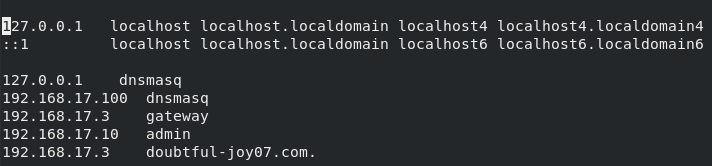
\includegraphics[width=0.95\textwidth]{data/dns-hosts-file.png}
  \caption{DNS-Einstellungen}
  \label{fig:DNSSettings}
\end{figure}

Die Funktion des \ac{DNS} kann mittels \texttt{nslookup}, zu sehen in \vref{fig:DNSNslookup}, oder über das Aufrufen des Frontends des Webservers, zu sehen in \vref{fig:Frontend}, überprüft werden.

\begin{figure}[htbp]
  \centering
  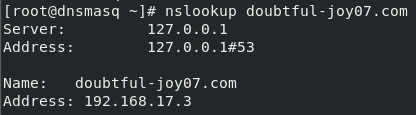
\includegraphics[width=0.95\textwidth]{data/dns-works-nslookup.png}
  \caption{Überprüfen des DNS mittels Namens}
  \label{fig:DNSNslookup}
\end{figure}

\begin{figure}[htbp]
  \centering
  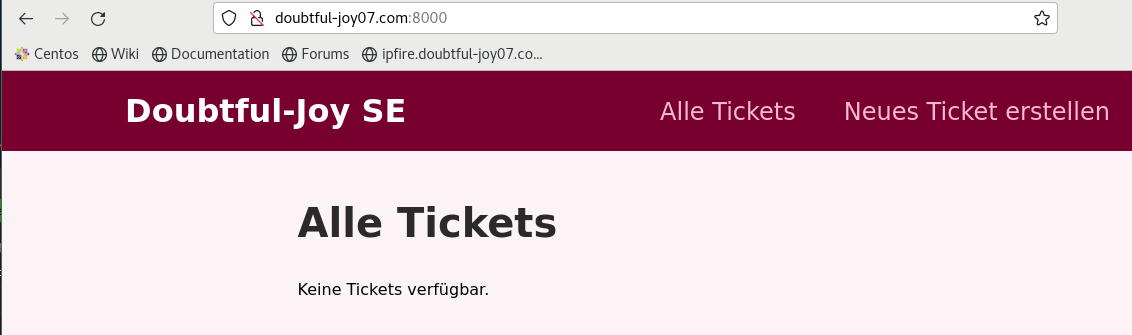
\includegraphics[width=0.95\textwidth]{data/dns-names-working.png}
  \caption{Aufrufen des Frontends mittels Name}
  \label{fig:Frontend}
\end{figure}


\subsection{Einrichtung des Datenbank-Servers}

Die Einrichtung eines Datenbank-Servers erfolgt mittels der Anleitung von Aaron Kili. \autocite{tecmint:PostgreSQLAndpgAdmin} Mit dieser wird PostGreSQL, ein \glqq{}leistungsstarkes, weit verbreitetes, quelloffenes, plattformübergreifendes und fortschrittliches objektrelationales Datenbanksystem\grqq{} \autocite{tecmint:PostgreSQLAndpgAdmin} und pgAdmin, ein \glqq{}fortschrittliches, quelloffenes, voll funktionsfähiges und webbasiertes Verwaltungs- und Managementwerkzeug\grqq{} \autocite{tecmint:PostgreSQLAndpgAdmin}, installiert.

Mittels des Webinterfaces, das pgAdmin bereitstellt, lässt sich eine Datenbank erstellen, zu sehen in \vref{fig:DBErstellung}. Der Name der Datenbank wird auf \glqq{}tickets\grqq{}, der Benutzername auf \glqq{}ticketadmin\grqq{} und das Passwort auf \glqq{}adminadmin\grqq{} festgelegt.

\begin{figure}[htbp]
  \centering
  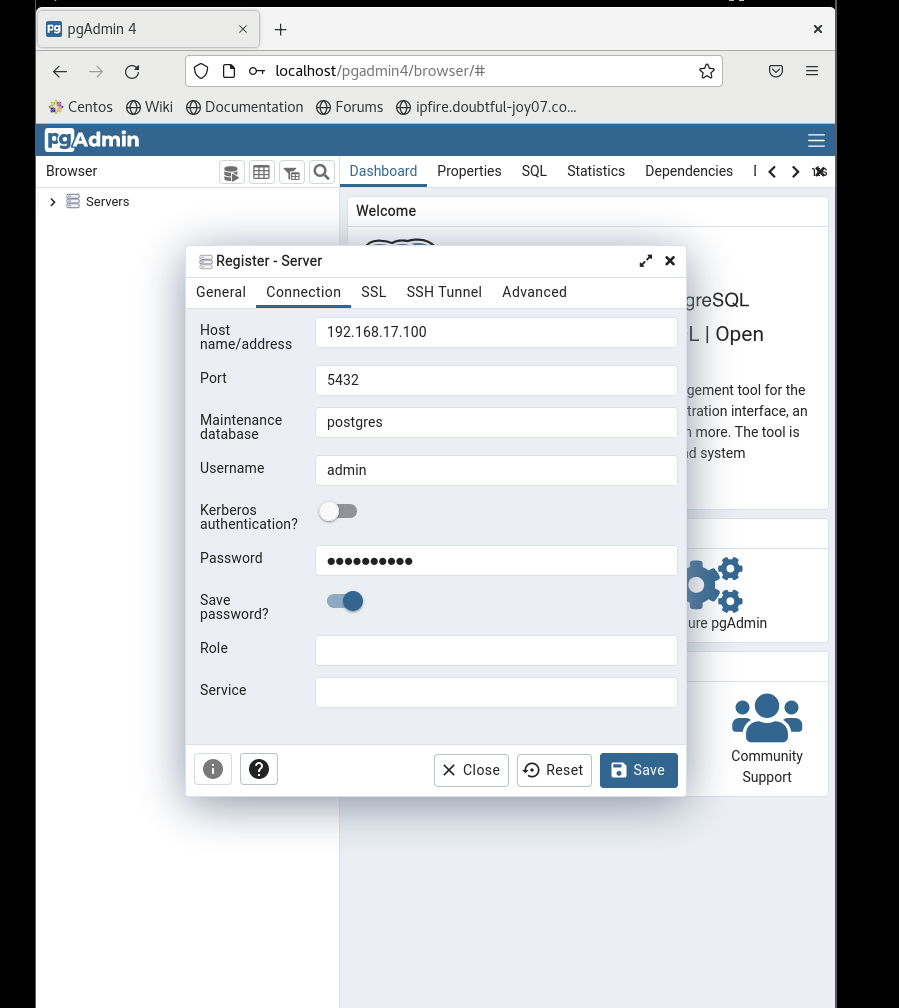
\includegraphics[width=0.95\textwidth]{data/PostGreSQL-Einrichtung.png}
  \caption{Einrichtung der Tickets-Datenbank}
  \label{fig:DBErstellung}
\end{figure}

Um die Kommunikation zwischen der Datenbank und dem Backend des Webservers zu erlauben, muss der Port 5432 freigegeben werden, zu sehen in \vref{lst:PGPortFreigabe}.

\begin{lstlisting}[language=bash,caption={Port-Freigabe einer CentOS-Firewall},label={lst:PGPortFreigabe}]
  # firewall-cmd --zone=public --add-port=5432/tcp --permanent
  # firewall-cmd --reload
\end{lstlisting}

Ebenso muss die \texttt{postgresql.conf} angepasst werden, so dass ein Zugriff von außerhalb überhaupt möglich ist. \autocite{vitux:PostgreSQL} Dies ist in folgendem \vref{lst:PostGreConfig} zu sehen.

\begin{lstlisting}[language=bash,caption={Einrichtung Zugriff PostGreSQL},label={lst:PostGreConfig}]
  # nano /var/lib/pgsql/data/postgresql.conf
  listen_addresses = '*'
\end{lstlisting}

Da im Front- und Backend Timestamps als Zahlen verwendet werden, muss die Tabelle noch geändert werden, damit kein \texttt{integer-out-of-range}-Fehler geworfen wird. Dies wird mittels der Befehls \texttt{ALTER TABLE} wie in \vref{lst:AlterSQL} umgesetzt.

\begin{lstlisting}[language=SQL,caption={Ändern der tickets-Tabelle},label={lst:AlterSQL}]
  ALTER TABLE order_detail ALTER COLUMN amount TYPE BIGINT;
\end{lstlisting}



\newpage
\section{Einrichtung Webserver}


\subsection{Einrichtung der CentOS-Installation}

Nach der Standard-Installation von CentOS 8 Stream wird das Netzwerk der \ac{VM} angepasst. Hier wird die IP-Adresse fest auf \texttt{192.168.244.10}, die Netzwerkmaske auf \texttt{255.255.255.0} und das Gateway auf \texttt{192.169.244.3} gesetzt. Außerdem wird der Port 8000 und Port 22 freigeben. Port 8000 dient dem Zugriff auf die Website von den beiden anderen Netzen aus und Port 22 erlaubt den \ac{SSH}-Zugriff des Admin-Pcs. Als Beispiel ist die Port-Freigabe für Port 8000 im \vref{lst:PortFreigabe} zu sehen.

\begin{lstlisting}[language=bash,caption={Port-Freigabe einer CentOS-Firewall},label={lst:PortFreigabe}]
  # firewall-cmd --zone=public --add-port=8000/tcp --permanent
  # firewall-cmd --reload
\end{lstlisting}

Abschließend wird Python3.10 installiert, um das Backend betreiben zu können.


\subsection{Einrichtung des Backends}

Das Backend wird mit Python3.10 umgesetzt. Hierfür wird mit Hilfe von FastAPI eine \ac{API} geschrieben, die verschiedene Routen bereitstellt, mit denen \ac{CRUD}-Anweisungen ausgeführt werden können. Außerdem dient das Backend auch gleich als Server für das Frontend, da es eben dieses bereitstellt.

Die benötigten Pakete können mittels \texttt{pip3.10 requirements.txt} installiert werden.


\subsection{Einrichtung des Frontends}

Für das Frontend wird die JavaScript-Softwarebibliothek React verwendet. Hier werden alle vom Kunden geforderten Anzeige und Bedienelemente implementiert. Da das Frontend bereits nach der Umsetzung gebaut und durch das Backend bereitgestellt wird, müssen keine Pakete installiert werden.



\section{Soll-Ist-Vergleich}

Der Zustand der abgelieferten Arbeit entspricht dem Soll-Zustand und somit den Kundenwünschen. Es werden alle Kriterien umgesetzt. Das Firewall-System, DHCP und DNS, Webserver und Datenbanksystem funktionieren einwandfrei.



\section{Abweichung zum Zeitplanung}

Der ursprüngliche Zeitplan, zu sehen in \vref{fig:GanttKlein}, bzw. \vref{fig:Gantt}, konnten nicht eingehalten werden. Es gab zwei Probleme:

\begin{itemize}
  \item Die Linux-Clients im IPFire Netz konnten keine Software installieren. \\
        Hier wurde vermutet, dass es an der Einrichtung der Firewall-Regeln lag, weswegen eine komplette Neuinstallation vorgenommen wurde. Dies hat unnötig Zeit gefressen. Die Lösung war dann, die System zu Hause einzurichten.
  \item Durch den Zeitverzug, den das erste Problem mit sich trug, konnte die Dokumentation nicht rechtzeitig fertiggestellt werden.
\end{itemize}

Das aktualisierte Gantt-Diagramm ist in klein in \vref{fig:GanttUpdateKlein} und groß im Anhang in \vref{fig:GanttUpdate} zu sehen.

\begin{figure}[htbp]
  \centering
  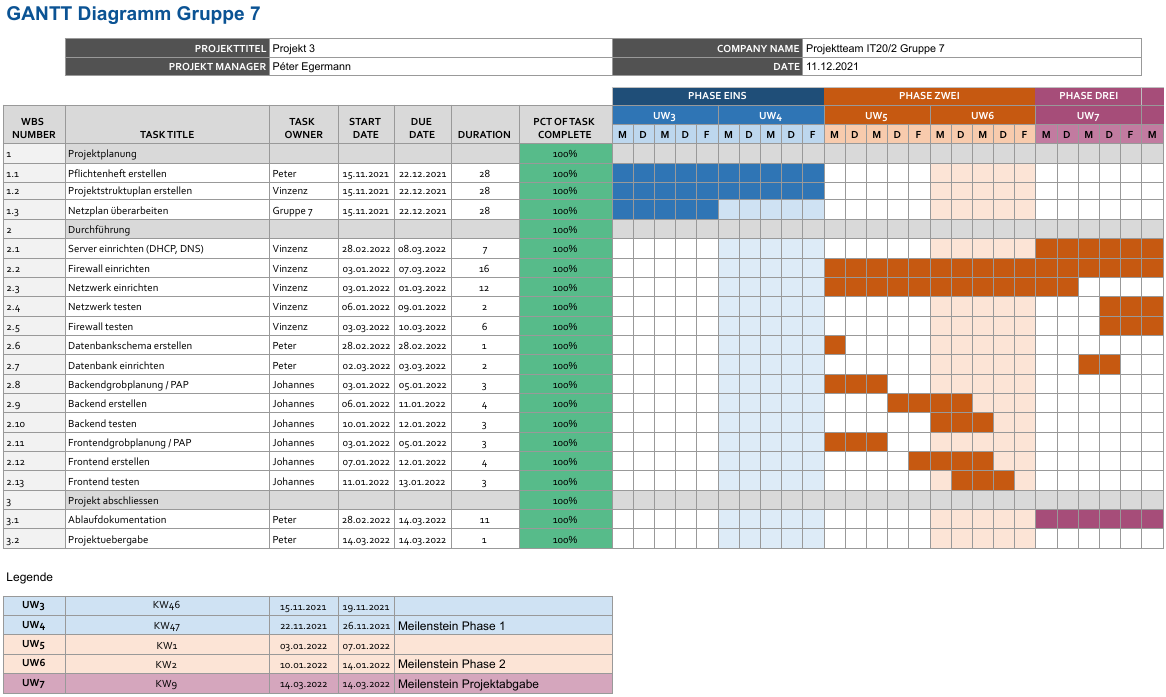
\includegraphics[width=0.95\textwidth]{data/Gantt_Abschluss.png}
  \caption{Gantt-Diagramm}
  \label{fig:GanttUpdateKlein}
\end{figure}



\section{Optimierungsvorschläge zur Projektrealisierung}

Das Projektteam IT20/2 Gruppe 7 besteht aus drei Anwendungsentwicklern, was die Sache deutlich erschwert hat. Hier wäre eine Überarbeitung der Gruppeneinteilung von Vorteil gewesen, so dass ein Team durch einen Systemintegrator und einen Anwendungsentwickler gebildet wird, wodurch sich gewisse Synergieeffekte ergeben könnten.


\newpage

%%% Abbildungsverzeichnis
\listoffigures
%%% Tabellenverzeichnis
\listoftables
%%% Codeverzeichnis
\lstlistoflistings
%%% Literaturverzeichnis
\printbibliography[keyword=Quelle,title={Literaturverzeichnis},heading=bibintoc]

\newpage

\appendix
\ihead{Anhang}



\chapter{Gantt-Diagramme}

\begin{figure}[h!]
  \centering
  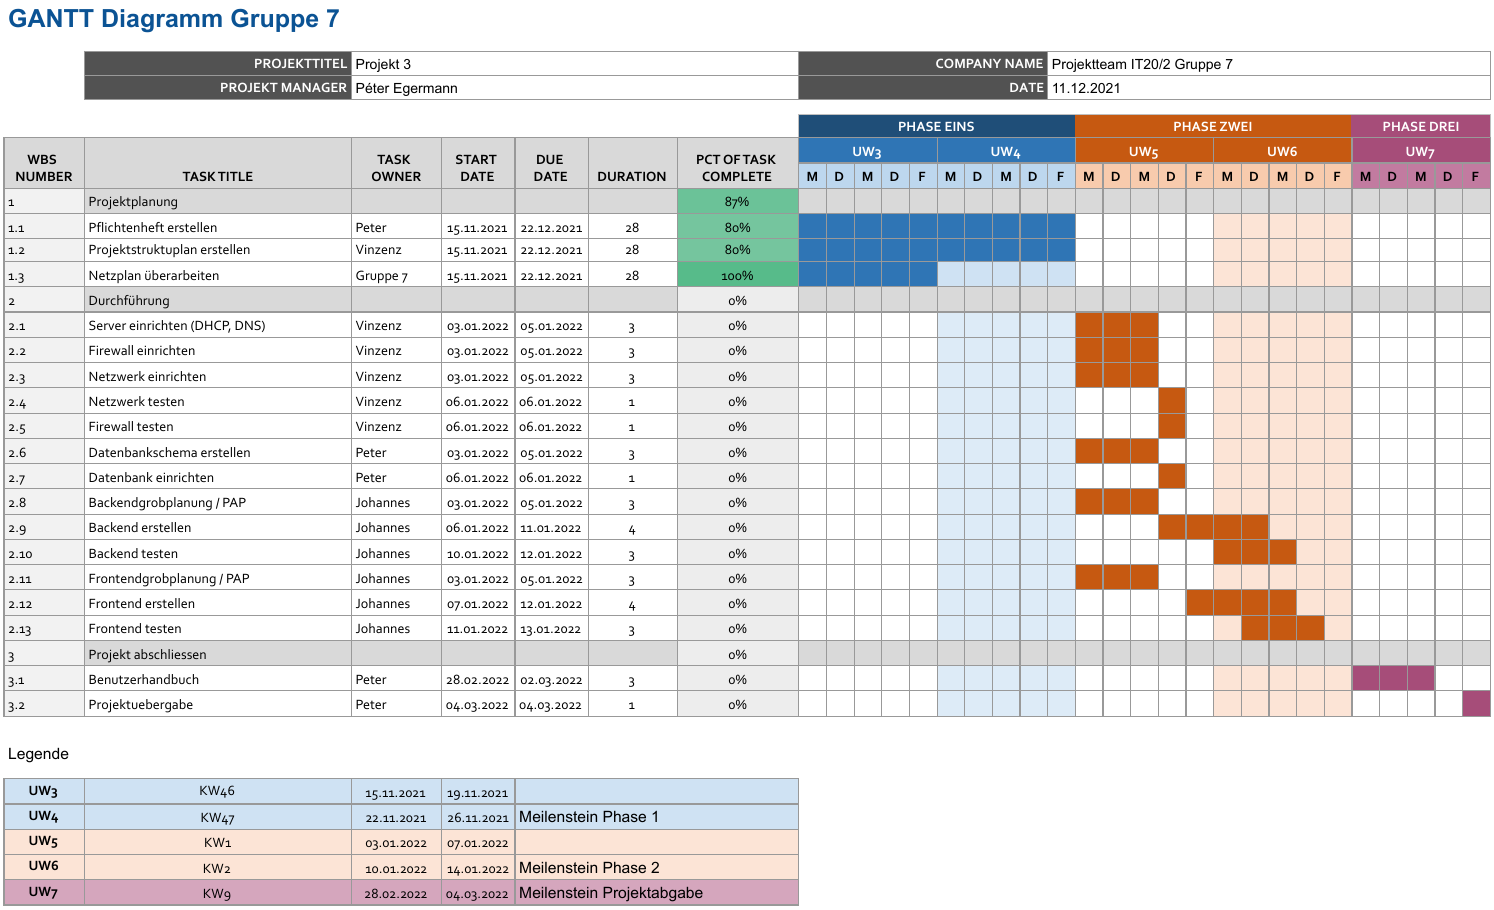
\includegraphics[angle=90,origin=c,width=0.75\textwidth]{data/Gantt.png}
  \caption{Gantt-Diagramm}
  \label{fig:Gantt}
\end{figure}

\newpage

\begin{figure}[h!]
  \centering
  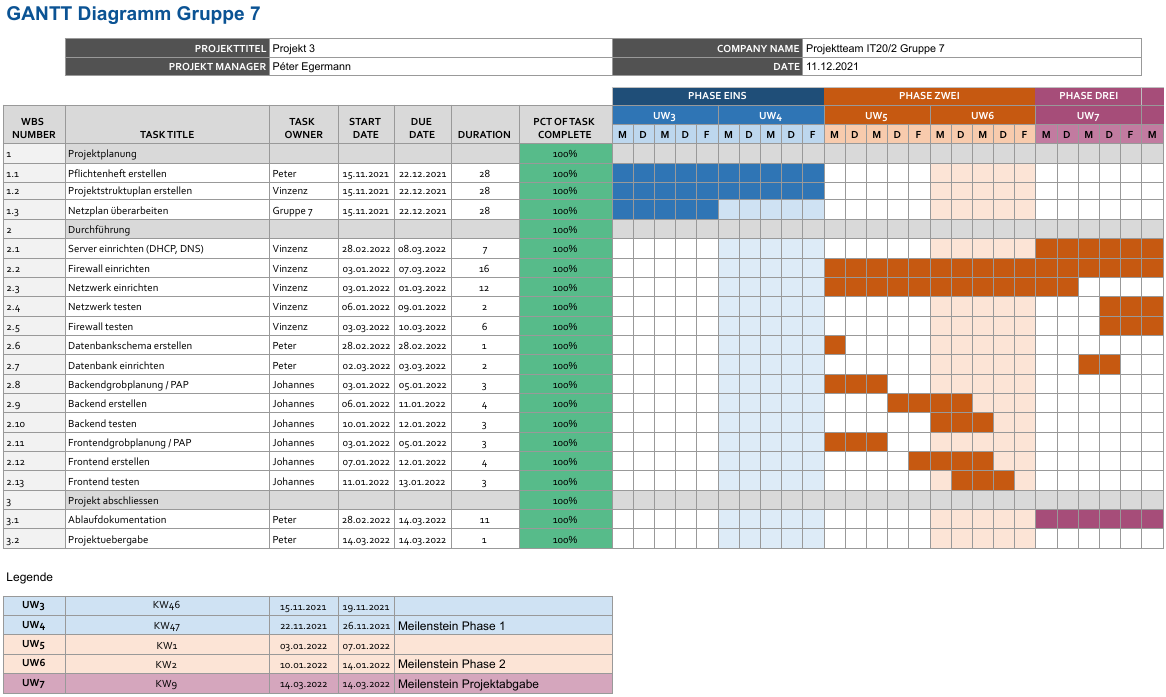
\includegraphics[angle=90,origin=c,width=0.75\textwidth]{data/Gantt_Abschluss.png}
  \caption{Update Gantt-Diagramm}
  \label{fig:GanttUpdate}
\end{figure}



\chapter{Netzwerkplan}

\begin{figure}[h!]
  \centering
  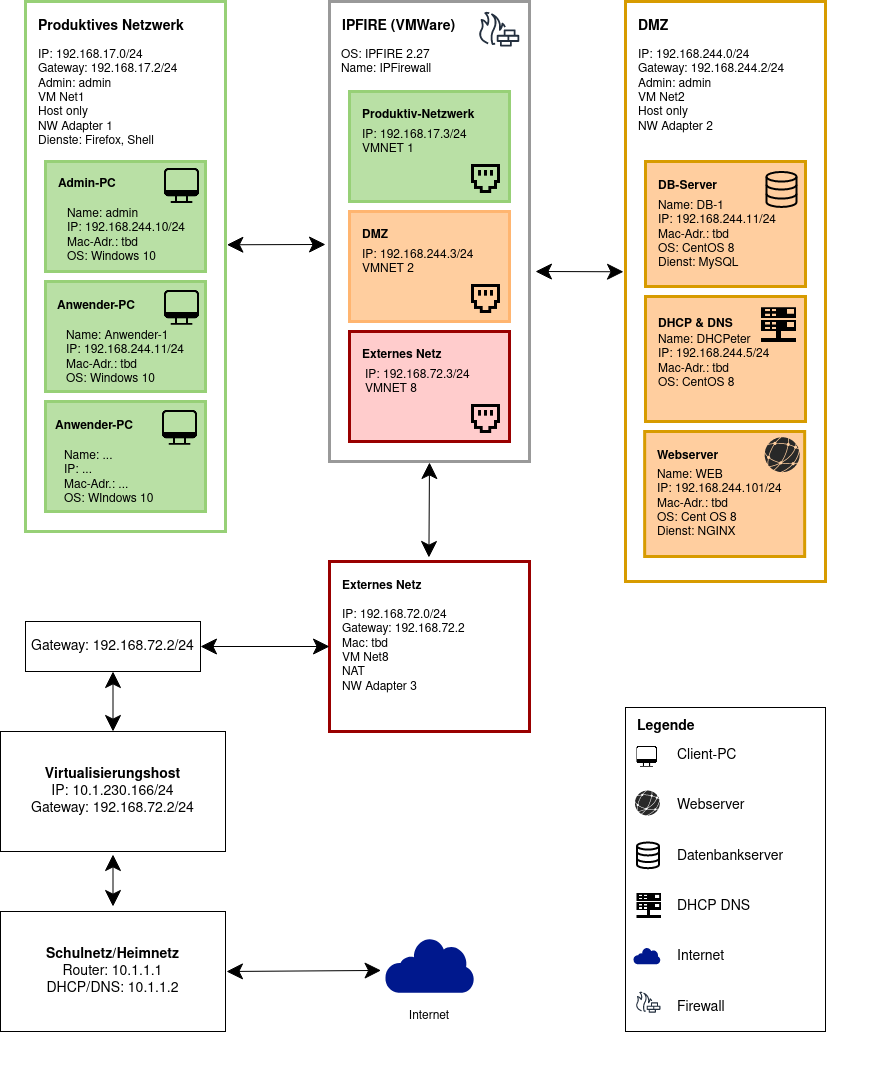
\includegraphics[width=0.95\textwidth]{data/Netzwerkplan.png}
  \caption{Netzwerkplan}
  \label{fig:Netzwerkplan}
\end{figure}

\end{document}
